
\chapter{Инфраструктура}

Для публикации приложения используются Amazon Web Services (AWS) - набор сервисов компании Amazon.

\section{Бэкенд инстансы}
\subsection{Старт новой машины}
	При автоматическом запуске машины мы можем передать очень маленькое количество информации, а именно, идентификатор AMI и User Data - небольшой набор инструкций, который будет выполнен после запуска чистой машины. В данной секции я расскажу о том, как при помощи этого небольшого количества данных можно запускать приложения.
	
	Для того, чтобы запустить чистую машину нам достаточно идентификатора AMI. Первоначально нами был выбран образ с CoreOS, т.к. планировалось запускать приложение внутри докер контейнера, а CoreOS как раз предназначена для таких случаев.
	
	После того как мы запустили чистую машину нам необходимо скачать наше приложение и всю необходимую инфраструктуру используя при этом только докер, т.к. в CoreOS кроме него больше ничего нет.
	
	Теоретически, всё приложение вместе с инфраструктурой можно было бы поместить внутрь одного докер образа, а при старте машины выполнить docker pull. Проблема такого подхода заключается в том, что при обновлении исходного кода приложения, что происходит очень часто, нам приходилось бы добавлять слой, что приводило бы к сильному росту размера образа. Так же при таком подходе нам не удалось бы обновить приложение не убивая докер контейнер, что привело бы к длительным перерывам в работе приложения при его обновлении.
	
	Учитывая это был применён несколько другой подход, при котором вся необходимая инфраструктура и настройки, которые меняются достаточно редко, помещаются в докер образ, а само приложение хранится в S3Bucket - облачном хранилище амазона. В такой ситуации при старте машины нам необходимо не только сделать docker pull образа с инфраструктурой, но и скачать наше приложение из S3 при помощи другого докер контейнера, т.к. утилиты для скачивания в CoreOS нет.
	
	В итоге мы получаем следующую User Data:
\begin{lstlisting}
[Unit]
Description=Kotlin web Demo backend Green
After=docker.service

[Service]
TimeoutStartSec=1800s
Restart=always
ExecStartPre=-/usr/bin/docker rm -f war-container-green
ExecStartPre=/usr/bin/docker run --name=war-container-green -v /wars docker-registry.labs.intellij.net/itops/aws-cli s3 cp s3://kotlin-web-demo-backend/green/WebDemoBackend.war /wars
ExecStartPre=/usr/bin/docker pull docker-registry.labs.intellij.net/kotlin/web-demo-backend
ExecStart=/usr/bin/docker run -m="1536m" --rm=true -e "LFS_NAME=kotlin.web.demo.backend" --name tomcat-green --volumes-from war-container-green -p 8080:20039 docker-registry.labs.intellij.net/kotlin/web-demo-backend

ExecStop=/usr/bin/docker stop tomcat-green
\end{lstlisting}

\subsection{Выбор типа EC2 instance}
	Одним из параметров конфигурации запуска инстанса на амазоне является его тип. Тип  инстанса определяет то, насколько мощный будет CPU, количество памяти и.т.д.. От типа машины зависит её стоимость - чем лучше машина, тем дороже она стоит. В таблице \ref{table:instance_types} приведены характеристики тех типов, которые рассматривались в качестве кандидатов.
	
	Как видно, CPU у ряда типов инстансов, а именно у t2 инстансов, помечены Burstable. Это - возможность машины временно увеличивать производительность CPU, тратя при этом кредиты CPU, которые копятся со временем, но теряются по истечении суток. В теории это должно быть удобно для приложений, у которых в среднем нагрузка мала, однако периодически она может возрастать, однако на практике с этим возникают проблемы, которые будут описаны далее.
	
\begin{table}[h]
	\centering
	\begin{tabular}{l|c|c|c}
		Type      & CPU Units    & Memory & Cost\\ \hline
		t2.small  & 1(Burstable) & 2GB    & \$0.026 hourly\\ \hline
		t2.medium & 2(Burstable) & 4GB    & \$0.052 hourly\\ \hline
		m3.medium & 3            & 3.75GB & \$0.070 hourly\\ \hline
		c4.large  & 8            & 3.75GB & \$0.116 hourly\\
	\end{tabular}
	\caption{Параметры интересующих нас типов амазоновских инстансов}
	\label{table:instance_types}
\end{table}
	
	Для сравнения производительности машин использовались два простых нагрузочных теста. В обоих тестах на сервер посылались запросы на исполнение "Hello, World!" программы. В первом случае запросы постоянно отправлялись из одного потока и измерялось время обработки каждого запроса. Во втором случае считалось максимальное количество потоков при котором сервер успевал исполнять программу (через 5 секунд после старта программа завершалась).
	
\begin{table}[h]
	\centering
	\begin{tabular}{l|c|c}
		Type      & Время обработки запроса    & Максимальное число потоков\\ \hline
		t2.small  & 0.5(Burst)/2.5             & 7(Burst)/1  \\ \hline
		t2.medium & 0.5(Burst)/2.5             & 15(Burst)/2 \\ \hline
		m3.medium & 1.2                        & 4           \\ \hline
		c4.large  & 0.5                        & 10          \\
	\end{tabular}
	\caption{Параметры интересующих нас типов амазоновских инстансов}
	\label{table:instance_types_performance}
\end{table}

	Из двух приведённых выше таблиц видно, что нам явно не подходят m3.medium инстансы, т.к. у них стабильно низкая мощность CPU.
	
	Намного интересней всё с t2 инстансами. Из таблицы \ref{table:instance_types_performance}	 видно, что они могут выдавать производительность даже больше чем c4.large инстансы, которые являются более дорогими. Однако есть очевидная проблема, которая заключается в том, что мы можем потратить все CPU кредиты. Данная проблема наиболее существенна при возникновении достаточно долгой большой нагрузки, т.к. общего числа накопленных кредитов может хватить максимум на пол часа работы машины при полном потреблении CPU. В такой ситуации одна машина перестанет справляться система автоматического масштабирования должна будет поднять новые, которые тоже будут типа t2. А это означает, что каждая поднятая машина в таких условиях сможет нормально работать только пол часа, после чего она станет почти бесполезной. 
	
	Также существует ещё одна неприятность, связанная с этим. Ресурсом, который мы активней всего тратим, является CPU, поэтому и наши метрики, которые отвечают за масштабирование, настроены на то, чтобы смотреть на потребление CPU. Когда у t2 ноды кончаются CPU кредиты уровень потребления CPU у неё не поднимается выше 20\%. Это приводит к тому, что согласно нашим метрикам, нагрузка на ноду мала, а значит и новые ноды поднимать не нужно. Данная ситуация является катастрофичной, т.к. сервера не смогут обрабатывать запросы в связи с тем, что они перегружены, а система масштабирования будет считать что всё нормально и ничего не предпринимать, что приведёт к неработоспособности приложения до тех пор, пока не спадёт нагрузка.
	
	Учитывая всё вышесказанное, можно сказать, что t2 ноды являются обладают очень хорошим соотношением мощности к цене, однако в сколь бы то ни было серьёзном приложении их использование представляется мне невозможным в связи с некоей непредсказуемостью поведения. Учитывая это, а так же тот факт , что m3.medium ноды обладают очень слабым процессором, в итоге были выбраны с4.large ноды.
\subsection{Подбор метрик}
	Как было сказано ранее, автоматическое масштабирование в амазоне основано на событиях Cloud Watch Alarm, каждое из которых говорит о том, что потребление определённого ресурса было больше/меньше определённого уровня.
	
	Как показал мониторинг нашего приложения, ресурс, который мы можем целиком потратить, один - процессорное время. Учитывая это были созданы соответствующие события:
\begin{itemize}
	\item Если среднее потребление CPU больше 80\% в течении 2 периодов по одной минуте, то увеличить количество инстансов в 2 раза, после чего подождать одну минуту перед следующим масштабированием.
	\item Если среднее потребление CPU меньше 40\% в течении 60 периодов по одной минуте, то уменьшить количество инстансов на 1, после чего подождать пять минут перед следующим масштабированием.
\end{itemize}
	Видно, что у данных метрик существенно различается время, которое мы ждём, перед тем как запускать новые ноды и перед тем как уничтожать старые ноды. Это позволяет нам избежать ситуации, при которой мы будем убивать только что поднятые ноды из-за того, что они уменьшили нагрузку, а потом поднимать их обратно, т.к. нагрузка возросла. Кроме того, при старте новой машины на амазоне мы оплачиваем один час её работы, что делает подобный подход ещё более осмысленным.
	
	Выбранная нами политика масштабирования является очень агрессивной, т.е. она очень мало ждёт перед поднятием новых нод и увеличивает количество нод в геометрической прогрессии. Это сделано для того, чтобы мы могли оперативно среагировать на резко увеличившуюся нагрузку. Недостатком такого подхода является то, что при случайном превышении порога, мы можем поднять много лишних машин, но в случае нашего приложения этот недостаток не проявляется, т.к. средняя нагрузка на наше приложение сильно меньше порога.
	
\subsection{Время запуска машины. Использование AMI}
	Время отклика приложения на рост нагрузки зависит не только от того, как мы настроили события в Cloud Watch, но и от того, сколько будет запускаться новый инстанс и сколько будет настраиваться на нём наша инфраструктура. 
	
	Со временем запуска нового инстанса мы сделать ничего не можем, это время более-менее постоянно и равно 1-2 минутам, а вот время настройки инфраструктуры мы можем пытаться уменьшить. В первоначальной версии это время составляло порядка 7 минут, что приводило к тому, что суммарное время отклика на рост нагрузки было больше 10 минут (2 минуты для срабатывания события, 2 минуты чтобы запустить машину, 7 минут чтобы настроить инфраструктуру). Основную часть этого времени мы тратили на скачивание образов докера, среди которых есть очень объёмный образ операционной системы.
	
	Единственный способ избежать скачивания докер образов это иметь эти докер образы локально. Это можно сделать если создать AMI работающей машины и использовать его для запуска новых машин. При таком подходе время настройки нашей инфраструктуры удалось сократить до нескольких минут, что привело к суммарному времени порядка 5 минут. 
\section{Инфраструктура с учётом обновлений}
При разработке любого приложения особое внимание следует уделить тому, как оно будет обновляться при изменениях и моё приложение не является исключением. Несмотря на то, что веб приложение должно обновляться достаточно легко, всё ж таки возникает несколько существенных проблем, а именно:
\begin{itemize}
	\item Свести время, в течении которого приложение будет неработоспособно, к минимуму.
	\item Обновить все части приложения (frontend и backend сервера) одновременно
\end{itemize}
\subsection{Green Blue deployment}
В результате перебора различных вариантов того как реализовать обновление приложения был выбран метод, известный как "Green-blue deployment", схема которого изображена на рис.\ref{fig:green_blue_deployment}.
\begin{figure}[h]
    \centering
    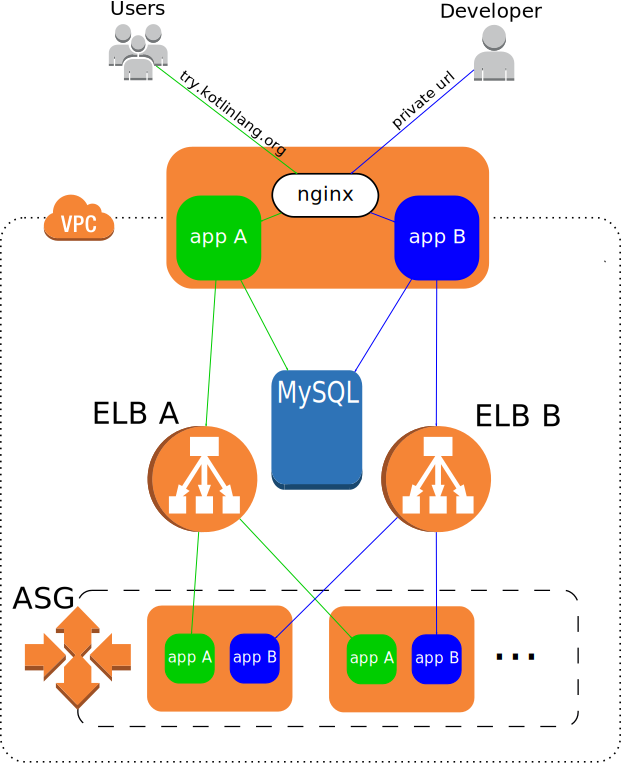
\includegraphics[scale=0.8]{green_blue_deployment} 
    \caption{Детальная схема устройства нашего приложения. Зелёным отмечено активное приложение, синим-пассивное}
    \label{fig:green_blue_deployment}
\end{figure}

	Основная идея данной схемы заключается в том, что существует две версии нашего приложения, активная и пассивная. Какое приложение является активным в данный момент определяется настройками nginx сервера. Все запросы к обоим приложениям идут на один и тот же сервер. Если запрос был отправлен на публичный адрес try.kotlinlang.org, то он будет перенаправлен активному приложению, а если он был отправлен на адрес, который известен только разработчикам, то он будет перенаправлен в пассивную ветку приложения.
	
	Какое приложение на данный момент является активным определяется исключительно настройками nginx, в результате чего мы можем легко поменять активное приложение с пассивным местами, что разрешает первую проблему. Вторая же проблема отпадает сама собой при такой схеме, т.к. мы можем целиком удалить пассивную ветку и создать её заново, что избавит нас от каких бы то ни было проблем синхронизации.
\subsection{Выбор стоимость-надёжность}
	Как видно из рисунка .\ref{fig:green_blue_deployment}, мы не дублируем никакие машины кроме ELB, которые необходимо дублировать, т.к. они умеют слушать только один порт и отправлять запросы тоже только на один порт. Это позволяет не иметь никаких дополнительных инстансов, а значит не тратить лишних денег.
	
	Пока всё работает как нужно такая схема является идеальной, но в случае возникновения ряда неполадок всё может стать очень плохо. Основная проблема в том, что два наших приложения разделяют один компьютер. На фронтенд сервере это не приводит ни к каким проблемам, т.к. каждое из приложений работает внутри своего докер контейнера и если одно из них ломается, то второе ничего не замечает, виртуализация, как никак.
	
	На бэкенд серверах всё было бы точно так же, если бы не одно но - бэкенд сервера постоянно проверяются на работоспособность балансировщиком нагрузки. Это приводит к тому, что если одно из наших приложений не отвечает по какой-то причине (что-то зависло в процессе публикации, мы выложили плохое приложение и.т.д), то данный компьютер будет остановлен, а на смену ему будет поднят новый. Если мы совсем невезучие, то с новым компьютером всё может повторится и компьютеры так и будут останавливаться - запускаться пока мы это не починим, а всё это время наш основной сайт не будет работать.
	
	Самым простым решением данной проблемы является создание двух ASG, что позволит запускать код активного и пассивного бэкендов на разных машинах, но в такой ситуации нужно тратить дополнительные деньги на работу инстансов пассивной ветки.